\documentclass[paper=a4, fontsize=11pt]{scrartcl} % A4 paper and 11pt font size

\usepackage[T1]{fontenc} % Use 8-bit encoding that has 256 glyphs
\usepackage{fourier} % Use the Adobe Utopia font for the document - comment this line to return to the LaTeX default
\usepackage[english]{babel} % English language/hyphenation
\usepackage{amsmath,amsfonts,amsthm} % Math packages
\usepackage{mathrsfs}  


\usepackage{sectsty} % Allows customizing section commands
\allsectionsfont{\centering \normalfont\scshape} % Make all sections centered, the default font and small caps

\usepackage{fancyhdr} % Custom headers and footers
\pagestyle{fancyplain} % Makes all pages in the document conform to the custom headers and footers
\fancyhead{} % No page header - if you want one, create it in the same way as the footers below
\fancyfoot[L]{} % Empty left footer
\fancyfoot[C]{} % Empty center footer
\fancyfoot[R]{\thepage} % Page numbering for right footer
\renewcommand{\headrulewidth}{0pt} % Remove header underlines
\renewcommand{\footrulewidth}{0pt} % Remove footer underlines
\setlength{\headheight}{13.6pt} % Customize the height of the header

\numberwithin{equation}{section} % Number equations within sections (i.e. 1.1, 1.2, 2.1, 2.2 instead of 1, 2, 3, 4)
\numberwithin{figure}{section} % Number figures within sections (i.e. 1.1, 1.2, 2.1, 2.2 instead of 1, 2, 3, 4)
\numberwithin{table}{section} % Number tables within sections (i.e. 1.1, 1.2, 2.1, 2.2 instead of 1, 2, 3, 4)

\setlength\parindent{0pt} % Removes all indentation from paragraphs - comment this line for an assignment with lots of text

\usepackage{graphicx}
\graphicspath{ {figures/} }
\usepackage{wrapfig}

%----------------------------------------------------------------------------------------
%	TITLE SECTION
%----------------------------------------------------------------------------------------

\newcommand{\horrule}[1]{\rule{\linewidth}{#1}} % Create horizontal rule command with 1 argument of height

\title{	
	\normalfont \normalsize 
	\textsc{ENS Cachan, M2 MVA} \\ [25pt] % Your university, school and/or department name(s)
	\horrule{0.5pt} \\[0.4cm] % Thin top horizontal rule
	\huge  Homework 2\\ % The assignment title
	\horrule{2pt} \\[0.5cm] % Thick bottom horizontal rule
}

\author{Sammy Khaliffe, Oussama Ennafii} % Your name

\date{\normalsize\today} % Today's date or a custom date

\begin{document}
	
	\maketitle % Print the title
	
	%----------------------------------------------------------------------------------------
	%	PROBLEM 1
	%----------------------------------------------------------------------------------------
	
	\section{Exercise 1.}
	
	1.  Let $f$ be a borelian function and $Y$ the resulting random variable from the algorithm:
	
	\begin{eqnarray*}
		\mathbb{E}[f(Y)] &=& \mathbb{E}_{\epsilon,B}[f(x \epsilon) \mathbb{1}_{B=1}+f(\frac{x}{\epsilon}) \mathbb{1}_{B=0}]\\
								  &=& \mathbb{E_{\epsilon}}[f(x \epsilon) \frac{1}{2}+f(\frac{x}{\epsilon}) \frac{1}{2}]\\
								  &=& \frac{1}{2} \int_{\mathbb{R}} [f(x \epsilon) +f(\frac{x}{\epsilon}) ] g(\epsilon) \mathbb{1}_{(-1,1)}(\epsilon)d\epsilon\\
								  &=& \frac{1}{2} \int_{|u|<|x|} f(u) g(\frac{u}{x}) \frac{du}{|x|} + \frac{1}{2} \int_{|u| > |x|} f(u) g(\frac{x}{u}) \frac{du |x|}{u^2}\\
	\end{eqnarray*}
	
	So if we denote by  $K(x,y)$ the p.d.f. of the proposal distribution:
	
	\begin{equation}
		K(x,y)=\frac{1}{2} g(\frac{y}{x}) \frac{1}{|x|} \mathbb{1}_{|y|<|x|} + \frac{1}{2} g(\frac{x}{y}) \frac{ |x|}{y^2} \mathbb{1}_{|y|>|x|} 
	\end{equation}
	
	2. Let $\pi$ be the invariant distribution :
	\begin{eqnarray*}
		\alpha(x,y) &=& min(1,\frac{\pi(y)}{\pi(x)} \frac{|y|}{|x|} \mathbb{1}_{|y|<|x|} + \frac{|y|}{|x|} \mathbb{1}_{|y|>|x|} )\\
						 &=& min(1,\frac{\pi(y)}{\pi(x)} |\epsilon| ) \mathbb{1}_{|y|<|x|}+  min(1,\frac{\pi(y)}{\pi(x)} \frac{1}{|\epsilon|} ) \mathbb{1}_{|y|>|x|}\\
	\end{eqnarray*}
	
	\begin{equation}
		\alpha(x,y)=min(1,\frac{\pi(y)}{\pi(x)} |\frac{y}{x}| ) 
	\end{equation}
	
	3. We implement this scheme for two distributions:
	\begin{itemize}
		\item[-] The hyperbolic secant distribution:
		$$f(x)=sech(\frac{\pi}{2}x)$$
		Its quantile function is:
		$$Q(p)=-\frac{2}{\pi} \text{\ log } ( \text{\ tan }(\frac{\pi}{2}))$$
		
		\item[-] The boltzman distribution of a quartic potential:
		
		$$V(x) \propto e^{-\frac{x-\mu)^2}{2 \sigma}(x-\mu)^2+\lambda(x-\mu)^4}$$
	\end{itemize}
	
	4. In the two cases, we estimate the mean with:
	
	$$\hat{\mu}_n=\frac{1}{N}\sum_{n=0}^{N}X_n$$
	
	We set:
	$$X_0:=2$$
	
	$$N:=5000$$
	
	$$\mu := 0$$
	
	and the other parameters to $1$.
	
	We get for the:
	\begin{itemize}
		\item[-] The logistic distribution:
		$$\hat{\mu}_n=-0.0308$$
		\item[-] The quartic potential well:
		$$\hat{\mu}_n=0.0131$$
	\end{itemize}
	
	5. We use here $5000$ samples.
	\begin{figure}
		\centering
		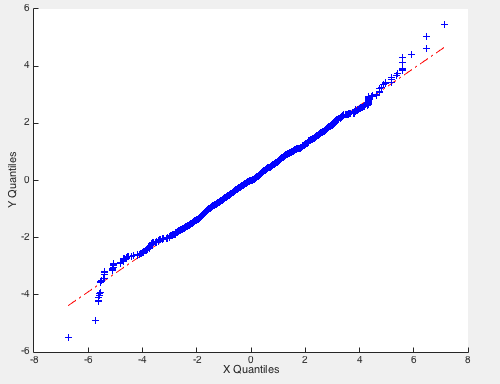
\includegraphics[width=0.25\textwidth]{qqplot}
		\caption{\label{fig:qqplot}QQ-plot comparing the MCMC invariant sequence to the true one}
	\end{figure}
	
	The two distrivutions concide well enough around the mean where we can sample with high praobability. However on the tails the two distributions differ.(c.f figure ~\ref{fig:qqplot})\\
	
	6. In figure ~\ref{fig:autocorr}, we can see that the autocorrelation coefficients decay very fast toward $0$. We can say then taht the burn in period of this scheme is small.
	\begin{figure}
		\centering
		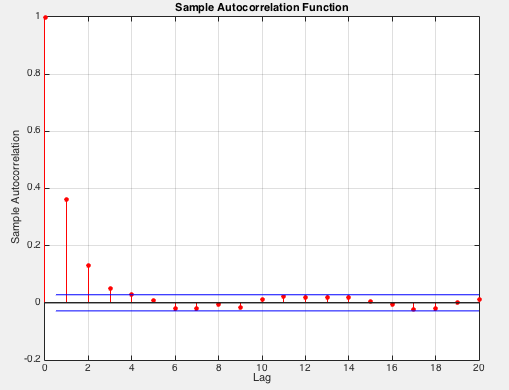
\includegraphics[width=0.25\textwidth]{autocorr}
		\caption{\label{fig:autocorr}Auto correlation plot for the secant hyperbolic distribution MCMC sample.}
	\end{figure}
	
	%----------------------------------------------------------------------------------------
	%	PROBLEM 2
	%----------------------------------------------------------------------------------------
	
	\section{Exercise 2.}
	
	1. When $f_0 \equiv 1$ , It is clear from step (b) that $X_n \in \{0,1\}, \forall n=1,\dots,+\infty$ and the transition kernel is a bernouli distribution.  We can see that this algorithm resembles the rejection algorithm. In fact, the step $(b)$ rejects $X_n$. The difference here is that the samples are not independent. \\
		
	2. Let $h$ be a borelian function. Set $n \in \mathbb{N}$ :
	\begin{eqnarray*}
		\mathbb{E}[h(X_{n+1} )|X_n ]&=&\mathbb{E}_{U_{n+1}}\int_{\mathbb{R}}h(x) f_0(x) \prod_{j=1}^{l}\mathbb{1}_{U_{n+1}^j \leq f_j(x)} dx\\
											&=& \int_{\mathbb{R}} \int_{\mathbb{R}^l}h(x) f_0(x) \prod_{j=1}^{l}\mathbb{1}_{u^j \leq f_j(x)} \frac{1}{f_j(X_n)} \mathbb{1}_{[0,f_j(X_n)]} d^lu dx\\
											&=& \int_{\mathbb{R}} h(x) f_0(x) \prod_{j=1}^{l} \int_{\mathbb{R}} \frac{1}{f_j(X_n)} \mathbb{1}_{0\leq u^j \leq min(f_j(x),f_j(X_n))} du^j  dx\\
											&=& \int_{\mathbb{R}} h(x) f_0(x) \prod_{j=1}^{l} \frac{min(f_j(x),f_j(X_n))}{f_j(X_n)} dx
	\end{eqnarray*}
	
	So the transition p.d.f. is:
	
	\begin{equation}
		K(x,y)=f_0(y) \prod_{j=1}^{l} \frac{min(f_j(y),f_j(x))}{f_j(x)}
	\end{equation}
	
	3. If we prove that $\pi$ is symmetric w.r.t. $K$ then $\pi$ would be invariant.
	
	\begin{eqnarray*}
		\pi(x)K(x,y)&=& f_0(x) \prod_{j=1}^{l} f_j(x) f_0(y) \prod_{j=1}^{l} \frac{min(f_j(y),f_j(x))}{f_j(x)}\\
						&=&  f_0(x) f_0(y) \prod_{j=1}^{l} min(f_j(y),f_j(x))\\
						&=& f_0(y) \prod_{j=1}^{l} f_j(y) f_0(x) \prod_{j=1}^{l} \frac{min(f_j(y),f_j(x))}{f_j(y)}\\
						&=& \pi(y)K(y,x)
	\end{eqnarray*}
	
	Let $\mathscr{A}$ be a borel set:
	
	\begin{eqnarray*}
		\int_{\mathscr{\mathbb{R} \times A}} 	\pi(x)K(x,y) &=& 	\int_{\mathscr{\mathbb{R} \times A}}  \pi(y)K(y,x) dx dy\\
																						&=& \int_{\mathscr{A }} \pi(y)( \int_{\mathscr{\mathbb{R}}} K(y,x) dx) dy\\
																						&=& \int_{\mathscr{A }} \pi(y) dy
	\end{eqnarray*}`
	
		%----------------------------------------------------------------------------------------
		%	PROBLEM 3
		%----------------------------------------------------------------------------------------
		
		\section{Exercise 3.}
	1. It is obviously not symmetric with two regions that are more probable and also separated. The problem that could rise then is that the chain stays too long in one region (possibly the right one) and thus we may not be aware of the local minima in the middle.(c.f. figure ~\ref{fig:density})\\
	
	\begin{figure}{R}
		\centering
		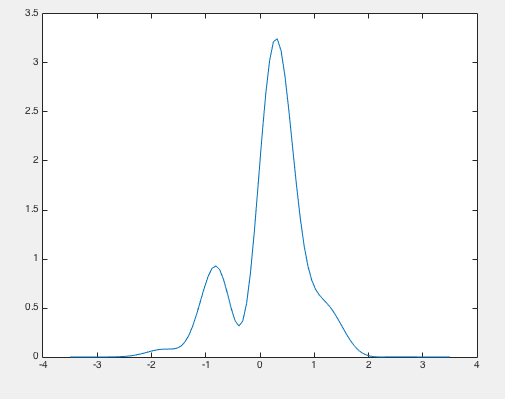
\includegraphics[width=0.25\textwidth]{density}
		\caption{\label{fig:density}The density shape.}
	\end{figure}
	2. We used two proposals:
	\begin{itemize}
		\item[(i)] An independent proposition kernel:
		$$K(x,y)=\mathscr{N}(x,0,1)$$
		\item[(ii)] A random walk proposition:
		$$Y_{n+1}=X_n+Z_{n+1}$$
		where $Z_n \sim \mathscr{N} (0,1)$
	\end{itemize}
	
	3. 
	\begin{wrapfigure}{R}{0.3\textwidth}
		\centering
		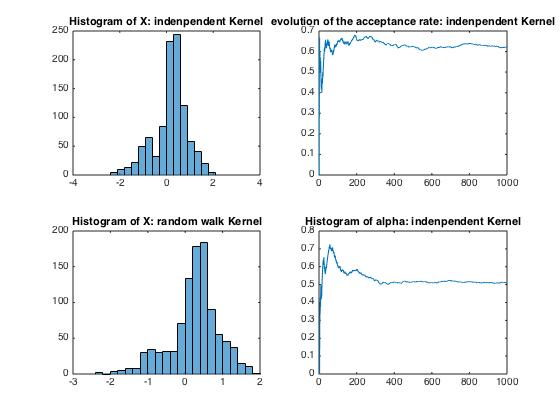
\includegraphics[width=0.3\textwidth]{comparison}
		\caption{\label{fig:comp}The comparison between the two samplers.}
	\end{wrapfigure}
	
	In this figure ~\ref{fig:comp}, we see that the independent proposition converges faster than the random walker. In average the acceptance ratio is $62\%$ for the first case and around $51\%$ in the second one. 
	
	4. For: $$N=100000$$
	and $$X_0=-2$$
	
	we run the indHM $10$ times, we get:
	$$\hat{\mu}_n \approx 0.19$$
	
	$$ \widehat{Var} _n \approx 0.46 $$
	 
	 and an estimate for the mode being $\approx 0.25$.
	  
	

\end{document}
	